\section{Mathematical Framework (Problem Formulation)}\label{sec:c3s2}
\kant[9-10]

This section builds on the material in \cref{sec:c3s1}, \cref{ch:4} and the prior work of \citet{ch3-10}; see also \citep{ch3-6,ch3-8}.

\begin{equation}\label{eq:c3s2-a}
  I = \int_{0}^{1}\!\!\int_{0}^{1} \frac{\sin(\pi x)\sin(\pi y)}{1+x^2+y^2}\,\mathrm{d}x\,\mathrm{d}y \approx \frac{1}{M}\sum_{m=1}^{M} h(\xi_m),
\end{equation}
with variance decreasing as
\begin{equation}\label{eq:c3s2-b}
  \operatorname{Var}\bigl[\hat I_M\bigr] = \frac{1}{M}\Bigl(\int h^2\,\mathrm{d}\mu - I^2\Bigr) = \mathcal{O}(M^{-1}).
\end{equation}

Equations~\eqref{eq:c3s2-a} and~\eqref{eq:c3s2-b} are used throughout the remainder of this section.

\kant[9-10]

\subsection{Quantitative behaviour}\label{sec:c3s2-q}
Results are collected in \cref{tab:c3s2} and visualised in \cref{fig:c3s2-f1}. Similar trends were reported in~\citep{ch3-12,ch3-2}.

\begin{table}[htbp]
\centering
\caption{Summary of measured quantities for experiment set \texttt{c3s2}.}\label{tab:c3s2}
\begin{tabular}{lrrr}
\toprule
Method & Score & Latency & Error \\
\midrule
Alpha & \num{54.6} & \SI{8.03}{\milli\second} & \num{3.456e-5} \\
Beta & \num{86.0} & \SI{4.61}{\milli\second} & \num{6.484e-3} \\
Gamma & \num{44.0} & \SI{5.28}{\milli\second} & \num{8.035e-5} \\
Delta & \num{42.8} & \SI{5.60}{\milli\second} & \num{7.864e-2} \\
Epsilon & \num{93.7} & \SI{7.24}{\milli\second} & \num{5.691e-2} \\
\bottomrule
\end{tabular}
\end{table}

\begin{figure}[htbp]
\centering
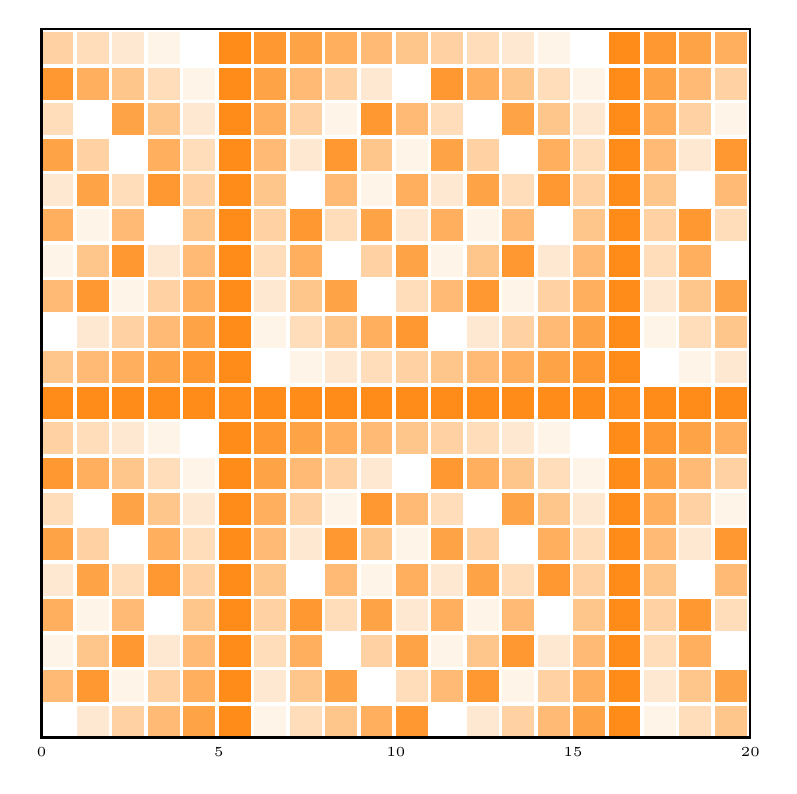
\begin{tikzpicture}[x=4.5mm,y=4.5mm]
\foreach \i in {0,...,19}{\foreach \j in {0,...,19}{\pgfmathtruncatemacro{\v}{mod(\i*2+\j*6+\i*\j,11)*9}
\fill[orange!\v!white](\i,\j)rectangle++(0.9,0.9);}}
\draw[thick](0,0)rectangle(20,20);
\foreach \i in {0,5,...,20}\node[below,font=\tiny]at(\i,0){\i};
\end{tikzpicture}
\caption{Generated figure for \texttt{c3s2-f1} (parameters $a=2$, $b=6$).}\label{fig:c3s2-f1}
\end{figure}

\lipsum[79-80]

\subsection{Implementation notes}\label{sec:c3s2-i}
The core routine is shown in \cref{lst:c3s2}; its complexity is $\mathcal{O}(N\log N)$ per iteration~\cite{ch3-9}.

\begin{lstlisting}[language=python,caption={Reference implementation for c3s2.},label={lst:c3s2}]
def conjugate_gradient(A, b, tol=1e-8, maxit=500):
    x = b * 0
    r = b - A @ x
    p = r.copy()
    for k in range(maxit):
        Ap = A @ p
        alpha = (r @ r) / (p @ Ap)
        x += alpha * p
        r_new = r - alpha * Ap
        if (r_new @ r_new) ** 0.5 < tol:
            break
        p = r_new + ((r_new @ r_new) / (r @ r)) * p
        r = r_new
    return x
\end{lstlisting}

\kant[9-11]
\begin{theorem}\label{thm:c3s2}
Let $A\in\mathbb{R}^{n\times n}$ be symmetric positive definite with condition number $\kappa$. Then the iteration converges and
$\lVert e_k\rVert_A \le 2\bigl(\tfrac{\sqrt\kappa-1}{\sqrt\kappa+1}\bigr)^k\lVert e_0\rVert_A$.
\end{theorem}
\begin{enumerate}[label=(\roman*)]
\item the bound in \cref{thm:c3s2} is sharp for some initial errors;
\item the constant $2$ cannot be improved in general;
\item preconditioning reduces the effective $\kappa$.
\end{enumerate}

\lipsum[76-76]
